\section{Approach}
This section discusses our approach to understand and elicit user requirements.

\subsection{Qualitative Analysis of Sensemaking}
We conducted two sets of observations to explore the characteristics of qualitative analysis of sensemaking activities. The purpose was twofold:
\begin{enumerate}
	\item To identify any unique characteristics of qualitative analysis in sensemaking studies that are different from those in general HCI research.
	\item To understand the process and tools used, and to identify any potential issues that can be addressed using visualization.
\end{enumerate}

Each set of observations includes both how an HCI researcher collected observation data when a participant was performing a sensemaking task, and the following data analysis session, during which the researcher used a qualitative method to analyze the collected data and gained a deep understanding of the participant's sensemaking process. We call our observations as \emph{meta observation} to differentiate them from the observations HCI researchers conducted. These HCI researchers are our target users. \autoref{fig:sp-meta-observation} illustrates the meta observation process.

\begin{figure}
 	\centering
 	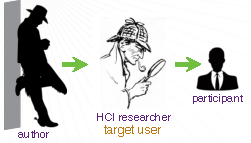
\includegraphics[width=.5\linewidth]{meta-observation}
 	\caption[Meta observation]{Meta observation. An HCI researcher conducts a qualitative study to understand a participant's sensemaking process. This study includes user observation and data analysis. We observe this study to explore its characteristics and identify potential support to HCI researchers -- our target users.}
 	\label{fig:sp-meta-observation}
\end{figure}

In the first meta observation, six participants were recruited and asked to do research online and select the smart watch they would like to purchase. The session stopped when the participant decided on the smart watch model, lasting between 30 to 45 minutes. These sessions were observed by a junior HCI researcher with limited qualitative analysis experience, and he recorded the sensemaking process by making notes on paper and screen recording. Interviews were conducted once the task was completed. Once all six observations were completed, the researcher conducted a \emph{thematic analysis} on the observation data, and the results were summarized in a two-page report. We interviewed the researcher after the report was finished to gain deeper understanding of his qualitative research process.

To ensure the qualitative analysis we observed was not biased, we conducted a second set of meta observations with a more experienced HCI researcher. One participant was tasked to plan a holiday for a fictitious family with particular needs. Two further participants were given the task to select a smart watch as described earlier. This researcher also made notes during the observation, and used thematic analysis to analyze the observation data.

To identify any unique features of qualitative analysis in sensemaking research, we conducted our own thematic analysis on the meta observation data. On completion, we discussed our findings with the two HCI researchers who participated in the meta observations. This led to a qualitative research process that aims to understand sensemaking, consisting of the following steps:

\begin{enumerate}
	\item \textbf{Study Design}. Decide the study setup including the sensemaking task, dataset, and data to capture based on the targeted research question.
	\item \textbf{Data Collection}. Capture the processes while the participants perform their sensemaking tasks. The collected data could include screen captures, think-aloud recordings, video recordings of participants' faces and gestures, and interview notes.
	\item \textbf{Transcription}. Transcribe video and audio recordings verbatim.
	\item \textbf{Coding}. Identify common themes in the transcripts and assign appropriate names or codes to them.
	\item \textbf{Categorization}. Group similar themes into more abstract categories.
	\item \textbf{Model}. Match the identified themes and categories to existing sensemaking models or design a new one, depending on the research question.
\end{enumerate}

Step 2 to 6 represent a progression on the semantics: each step takes the output from the previous step as input, and produces an outcome with richer semantics. This is similar to the four layers of visual analytic activities in the Gotz and Zhou's model (\autoref{sec:lr-analytic-provenance-model}), but targeting a different aspect: the former focuses on the sensemaking model and theory, whereas the latter focuses on user activities. In summary, we did not discover any unique characteristics of qualitative analysis for sensemaking. This implies the approach and tool we developed for sensemaking are likely to be applicable to qualitative analysis intended for other purposes. Our study did equip us with detailed knowledge about the actual qualitative analysis process, which informed the design of our visualization tool.

\subsection{Requirements}
A participatory design session with the two HCI researchers involved in the meta observations was followed up to elicit requirements for the tool that aims to facilitate the existing analysis process. The session discussed possible tool features and designs to address them. The requirements are presented as follows and the design ideas are described in \autoref{sec:sp-design}.
%Our meta thematic analysis led to these requirements:

\begin{enumerate}
	\item \textbf{Thematic analysis support}. This is the analysis method used in both our meta observations and the two sensemaking observations. It also shares many characteristics with other popular qualitative research analysis methods such as grounded theory.

	\item \textbf{Transcription and Coding efficiency}. All aforementioned steps from 2 to 6 are time-consuming; however, \emph{transcription} and \emph{coding} are where a visualization tool can potentially make the most difference. Their lengths largely depend on the efficiency of the tools employed in these steps. \emph{Data collection} primarily depends on the task's completion time and the number of participants. Also, transcription and coding are not as abstract or semantically rich as \emph{categorization} and \emph{model}, making it more feasible to provide automated support.

	%\setcounter{listnum}{\theenumi}
%\end{enumerate}
%
%The participatory design session with HCI researchers led to these requirements:
%
%\begin{enumerate}
%	\setcounter{enumi}{\thelistnum}
	\item \textbf{Existing workflow integration}. The tool should maintain the way researchers currently work and ideally works together with other software packages already used in the analysis workflow.
	\item \textbf{Non-intrusiveness}. The tool should not distract participants or affect their behaviors during the sensemaking tasks.
	\item \textbf{Scalability}. The tool should support reasonably long sensemaking sessions with a duration up to an hour or two.
	\item \textbf{Lightweight}. The tool should be lightweight and support multiple operating systems.

\end{enumerate}